\documentclass[letterpaper]{article}
\usepackage[square,sort,comma,numbers]{natbib}
\usepackage{array}
%====================================================================%
../../../../tex/scufftex.tex
\graphicspath{{figures/}}
\renewcommand{\wt}{\widetilde}
\newcommand{\vbCSlash}{\backslash\hspace{-0.085in}\vb C}
\newcommand{\JSlash}{\backslash\hspace{-0.085in}J}

%------------------------------------------------------------
%------------------------------------------------------------
%- Special commands for this document -----------------------
%------------------------------------------------------------
%------------------------------------------------------------

%------------------------------------------------------------
%------------------------------------------------------------
%- Document header  -----------------------------------------
%------------------------------------------------------------
%------------------------------------------------------------
\title {Implicit handling of multilayered material substrates
        in full-wave {\sc scuff-em} calculations
       }
\author {Homer Reid}
\date {August 16, 2017}

%------------------------------------------------------------
%------------------------------------------------------------
%- Start of actual document
%------------------------------------------------------------
%------------------------------------------------------------

\begin{document}
\pagestyle{myheadings}
\markright{Homer Reid: Implicit substrates in full-wave {\sc scuff-em}}

\maketitle

\tableofcontents

%====================================================================%
%====================================================================%
%====================================================================%
\newpage
\section{Overview}

In a 
previous memo\footnote{``Implicit handling of multilayered dielectric
substrates in -wave {\sc scuff-static}''} I
considered {\sc scuff-static} electrostatics calculations
in the presence of a multilayered dielectric substrate.
In this memo I extend that discussion to the case of
\textit{full-wave} (i.e. nonzero frequencies beyond the
quasistatic regime) scattering calculations in the
{\sc scuff-em} core library.

%%%%%%%%%%%%%%%%%%%%%%%%%%%%%%%%%%%%%%%%%%%%%%%%%%%%%%%%%%%%%%%%%%%%%%
%%%%%%%%%%%%%%%%%%%%%%%%%%%%%%%%%%%%%%%%%%%%%%%%%%%%%%%%%%%%%%%%%%%%%%
%%%%%%%%%%%%%%%%%%%%%%%%%%%%%%%%%%%%%%%%%%%%%%%%%%%%%%%%%%%%%%%%%%%%%%
\subsubsection*{Substrate geometry}

As shown in Figure \ref{SubstrateGeometryFigure}, I consider
a multilayered substrate consisting of $N$ material layers
possibly terminated by a perfectly-conducting ground plane.
The uppermost layer (layer 1) is the infinite half-space
above the substrate.
The $n$th layer
has relative permittivity and permeability $\epsilon_n,\mu_n$,
and its lower surface lies at $z=z_n$.
The ground plane, if present,
lies at $z\equiv z\subt{N}\equiv z\subt{GP}$.
If the ground plane is absent, layer $N$ is an
infinite half-space\footnote{As in the electrostatic case,
this means that a finite-thickness substrate consisting of
$N$ material layers is described as a stack of $N+1$ layers
in which the bottommost layer is an infinite vacuum half-space.}
($z\subt{N}=-\infty$).
%####################################################################%
%####################################################################%
%####################################################################%
\begin{figure}[!]
\begin{center}
\resizebox{\textwidth}{!}{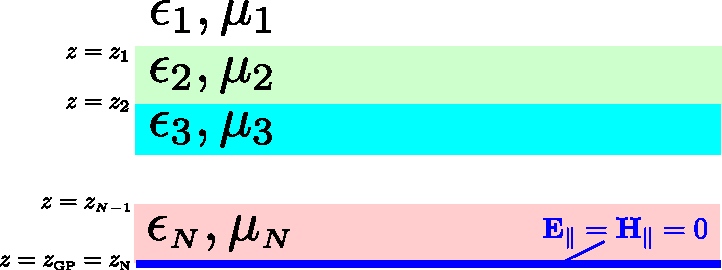
\includegraphics{MultilayerSubstrate.pdf}}
\caption{Geometry of the layered substrate.
The $n$th layer 
has relative permittivity and permeability $\epsilon_n,\mu_n$,
and its lower surface lies at $z=z_n$. The ground plane, if present,
lies at $z=z\subt{GP}.$
}
\label{SubstrateGeometryFigure}
\end{center}
\end{figure}
%####################################################################%

%%%%%%%%%%%%%%%%%%%%%%%%%%%%%%%%%%%%%%%%%%%%%%%%%%%%%%%%%%%%%%%%%%%%%%
%%%%%%%%%%%%%%%%%%%%%%%%%%%%%%%%%%%%%%%%%%%%%%%%%%%%%%%%%%%%%%%%%%%%%%
%%%%%%%%%%%%%%%%%%%%%%%%%%%%%%%%%%%%%%%%%%%%%%%%%%%%%%%%%%%%%%%%%%%%%%
\subsubsection*{Mechanics of implementation in {\sc scuff-em}}

The mechanics of implementing support for multilayer substrates
in {\sc scuff-em} boils down to a two-step process:
\begin{itemize}
 \item Devise a numerical scheme for computing the
       substrate contribution $\bmc G\sups{subs}$
       to the full dyadic Green's function (DGF)
       $\bmc G\equiv \bmc G^0 + \bmc G\sups{subs}.$
       The quantity $\bmc G(\vb x, \vb x^\prime)$
       describes the fields at $\vb x$ due to
       point sources at $\vb x^\prime$, including
       both the direct vacuum contributions ($\bmc G^0$)
       and the contributions due to scattering from the
       substrate $(\bmc G\sups{subs}).$
 \item Incorporate the substrate DGF correction $\bmc G\sups{subs}$ into
       the existing {\sc scuff-em} framework for
       evaluating 4-dimensional integrals of the form
       $\Vmv{\vb b_\alpha}{\bmc G}{\vb b_\beta}$
       where $\vb b_{\alpha,\beta}$ are RWG basis functions.
       To achieve reasonable efficiency, this will require
       combining a variety of numerical computational 
       techiques, including look-up tables, interpolation schemes,
       and asymptotic expansions.
\end{itemize}

In this memo I will discuss methods for attacking
both of these challenges.

%####################################################################%
%####################################################################%
%####################################################################%
\newpage
\section{Evaluation of substrate Green's-function correction}

My calculation of $\bmc G\sups{subs}$ proceeds in two stages:
%====================================================================%
\begin{itemize}
 \item Obtain expressions for the 2D Fourier transform of the
       substrate GF correction, $\wt{\bmc G}\sups{subs}(\vb q)$.
       I consider two separate ways of doing this:
       %====================================================================%
       \begin{itemize}
         \item By using surface-integral-equation methods to solve
               a scattering problem to determine effective 
               surface-current densities induced on material interfaces
               by radiating point sources (Section \ref{SurfaceCurrentSection}).
         \item By resolving the fields radiated by point sources
               into superpositions of plane waves, then considering the 
               reflection of each individual plane wave from the 
               multilayer substrate (Section \ref{PlaneWaveSection}).
       \end{itemize}
       %====================================================================%
         
 \item Evaluate the 2D integrals over the $\vb q$ variable
       to effect the inverse Fourier transform from momentum space
       to real space,
       $\wt{\bmc G}\sups{subs}(\vb q) \to \bmc G\sups{subs}(\vbrho).$
       This calculation proceeds in two stages:
       \begin{itemize}
         \item Use the known structure of $\wt{\bmc G}(\vb q)$
               to reduce 2D integrals over $\vb q$ to 1D integrals over $q_z$
               (Section \ref{TwoDToOneDSection}).
         \item Devise numerical quadrature methods for evaluating the
               $q_z$ integrals, including efficient and accurate handling
               of integrable singularities and undamped oscillatory integrands
               (Section \ref{OneDIntegralSection}).
       \end{itemize}
\end{itemize}
%====================================================================%

%%%%%%%%%%%%%%%%%%%%%%%%%%%%%%%%%%%%%%%%%%%%%%%%%%%%%%%%%%%%%%%%%%%%%%
%%%%%%%%%%%%%%%%%%%%%%%%%%%%%%%%%%%%%%%%%%%%%%%%%%%%%%%%%%%%%%%%%%%%%%
%%%%%%%%%%%%%%%%%%%%%%%%%%%%%%%%%%%%%%%%%%%%%%%%%%%%%%%%%%%%%%%%%%%%%%
\subsection{Derivation of momentum-space DGF, take 1: Effective surface-current picture}
\label{SurfaceCurrentSection}

%####################################################################%
%####################################################################%
%####################################################################%
\begin{figure}[t]
\begin{center}
\resizebox{\textwidth}{!}{\includegraphics{MultilayerSubstrateWithSurfaceCurrents.pdf}}
\caption{Effective surface-current approach to treatment of
multilayer substrate. External field sources induce a distribution
of electric and magnetic surface currents $\bmc S_n={\vb K_n \choose \vb N_n}$
on the $n$th material interface, and the fields radiated by these
effective currents account for the disturbance presented by
the substrate.}
\label{SurfaceCurrentFigure}
\end{center}
\end{figure}
%####################################################################%
%####################################################################%
%####################################################################%
One way to account for the disturbance produced by the
substrate is to consider the effective tangential electric and magnetic
surface currents $\vb K$ and $\vb N$ induced on the interfacial 
layers by the external field sources 
(Figure \ref{SurfaceCurrentFigure}). This is the direct extension
to full-wave problems of the formalism I used in the electrostatic
case, and it comports well with the spirit of
surface-integral-equation methods.

More specifically, on the material interface layer at $z=z_n$
I have a four-vector surface-current density $\bmc S_n(\vbrho)$,
where $\vbrho=(x,y)$ and the components of $\bmc S$ are
%====================================================================%
\numeq{SnDef}
{ \bmc S_n(\vbrho)=
  \left(\begin{array}{c}
     K_x(\vbrho) \\ K_y(\vbrho) \\ N_x(\vbrho) \\ N_y(\vbrho)
  \end{array}\right).
}
%====================================================================%

\paragraph{Fields in layer interiors.} 
I will adopt the convention that the lower (upper) bounding surface
for each region is the positive (negative) bounding surface
for that region in the usual sense of {\sc scuff-em} regions and
surfaces (in which the sign of a \{surface,region\} pair $\{\mc S, \mc R\}$ 
is the sign with which surface currents on $\mc S$ contribute to
fields in $\mc R$).
Thus, at a point $\vb x=(\vbrho,z)$ in the interior of layer $n$
($z_{n-1} > z > z_n$), the six-vector of total fields
$\bmc F=\hbox{\scriptsize{
 $\left(\begin{array}{c} \vb E \\ \vb H\end{array}\right)$}}
$
reads
%====================================================================%
\numeq{Fn}
{  \bmc F_n(\vbrho, z)
  =
  - \bmc G^n(z_{n-1}) \star \bmc S_{n-1}
  + \bmc G^n(z_{n}) \star \bmc S_{n}
  + \bmc F\sups{ext}_n(\vbrho, z)
}
%====================================================================%
where $\bmc F\sups{ext}_n$
are the externally-sourced (incident) fields
due to sources in layer $n$, $\bmc G^n$ is the homogeneous dyadic
Green's function for material layer $n$, and $\star$
is shorthand for the convolution operation
%====================================================================%
\numeq{ConvolutionDef}
{
``\bmc F(\vbrho, z) \equiv \bmc G(z^\prime) \star \bmc S''
   \quad \Longrightarrow \quad 
    \bmc F(\vbrho,z) = 
    \int
      \bmc G(\vbrho-\vbrho^\prime,z-z^\prime)\cdot \bmc S(\vbrho^\prime)
    d\vbrho^\prime
}
%====================================================================%
where the integral extends over the entire interfacial plane.
I will evaluate convolutions of this form using the
2D Fourier representation of $\bmc G$:
%====================================================================%
\begin{subequations}
\begin{align}
  \bmc G^n(\vbrho, z)
 &=
  \int \frac{d^2 \vb q}{(2\pi)^2}
  \wt{\bmc G^n}(\vb q, z) e^{i\vb q \cdot \vbrho}
\\
%--------------------------------------------------------------------%
   \wt{\bmc G^n}(\vb q, z)
&= \frac{1}{2}
   \left(\begin{array}{cc}
      -\frac{\omega \mu_0 \mu_n}{q_{zn}} \wt{\vb G}^\pm
    & +\wt{\vb C}^\pm 
    \\[5pt]
      -\wt{\vb C}^\pm
    & -\frac{\omega \epsilon_0 \epsilon_n}{q_{zn}} \wt{\vb G}^\pm
   \end{array}\right)e^{iq_z |z|}
\\[10pt]
%--------------------------------------------------------------------%
   \wt{\vb G}^\pm(\vb q, k)
&= \left(\begin{array}{ccc}
   1 & 0 & 0 \\[2pt] 0 & 1 & 0 \\[2pt] 0 & 0 & 1
   \end{array}\right)
   -
   \frac{1}{k^2}
   \left(\begin{array}{ccc}
    q_x^2    & q_xq_y       & \pm q_x q_z \\[2pt]
    q_y q_x  & q_y^2        & \pm q_y q_z \\[2pt]
 \pm q_z q_x  & \pm q_z q_y  & q_z^2 
   \end{array}\right)
\\[10pt]
%--------------------------------------------------------------------%
   \wt{\vb C}^\pm(\vb q, k)
&=
   \left(\begin{array}{ccc}
   0           & \mp 1     &    +q_y/q_z \\[2pt]
   \pm 1       & 0         &    -q_x/q_z \\[2pt]
  -q_y/q_z     & +q_x/q_z  &           0
  \end{array}\right)
\end{align}
\label{GFourier}
\begin{equation}
  k_n\equiv \sqrt{\epsilon_0 \epsilon_n \mu_0 \mu_n}\cdot \omega,
  \qquad 
  q_z \equiv \sqrt{k^2 - |\vb q|^2},
 \qquad 
  \pm = \text{sign} z.
\end{equation}
\end{subequations}
%====================================================================%
\noindent With this representation, convolutions like (\ref{ConvolutionDef})
become products in Fourier space:
%====================================================================%
\begin{align*}
\bmc G(z^\prime)\star \bmc S=
 \bmc F(\vbrho, z)
&=\int \frac{d^2 \vb q}{(2 \pi)^2} \wt{\bmc F}(\vb q,z) e^{i\vb q \cdot \vbrho},
\qtq{with}
 \wt{\bmc F(\vb q,z)}=\wt{\bmc G}(\vb q,z-z^\prime)\wt{\bmc S}(\vb q)
\end{align*}
%====================================================================%

\paragraph{Surface currents from incident fields.}

To determine the surface currents induced by given incident-field
sources, I apply boundary conditions.
The boundary condition at $z=z_n$ is that the tangential $\vb E, \vb H$
fields be continuous: in Fourier space, we have
%====================================================================%
\numeq{BCEquation}
{ \wt{\bmc F}_{\parallel}(\vb q, z=z_n^+)
 =\wt{\bmc F}_{\parallel}(\vb q, z=z_n^-)
}
The fields just \textbf{above} the interface $(z\to z_n^+)$ receive
contributions from three sources:
%====================================================================%
\begin{itemize}
 \item Surface currents at $z=z_{n-1}$, which contribute with
       a minus sign and via the Green's function for region $n$;
 \item Surface currents at $z=z_{n}$, which contribute with
       a plus sign and via the Green's function for region $n$; and
 \item external field sources in region $n$.
\end{itemize}
%====================================================================%
The fields just \textbf{below} the interface $(z=z_n^-)$ receive
contributions from three sources:
%====================================================================%
\begin{itemize}
 \item Surface currents at $z=z_{n}$, which contribute with
       a minus sign and via the Green's function for region $n+1$;
 \item Surface currents at $z=z_{n+1}$, which contribute with
       a plus sign and via the Green's function for region $n+1$; and
 \item external field sources in region $n+1$.
\end{itemize}
%====================================================================%
Then equation (\ref{BCEquation}) reads
%====================================================================%
\begin{align*}
&
-\wt{\bmc G^n}_{\parallel}(z_n-z_{n-1})\cdot \wt{\bmc S}_{n-1}
+\wt{\bmc G^n}_{\parallel}(0^+) \cdot \wt{\bmc S}_{n}
+\wt{\bmc F}\sups{ext}_{n\parallel}(z_n)
\\
&\qquad=
-\wt{\bmc G^{n+1}}{\parallel}(0^-) \cdot \wt{\bmc S}_{n}
+\wt{\bmc G^{n+1}}{\parallel}(z_n-z_{n+1})\cdot \wt{\bmc S}_{n+1}
+\wt{\bmc F}\sups{ext}_{n+1\parallel}(z_n)
\end{align*}
or
%====================================================================%
\numeq{MSFSlice}
{
  \vb M_{n,n-1}  \cdot \wt{\bmc S}_{n-1}
 +\vb M_{n,n}    \cdot \wt{\bmc S}_{n}
 +\vb M_{n,n+1}  \cdot \wt{\bmc S}_{n+1}
 =  \wt{\bmc F}\sups{ext}_{n+1\parallel}(z_n)
   -\wt{\bmc F}\sups{ext}_{n\parallel}(z_n)
}
%====================================================================%
with the $4\times 4$ matrix blocks\footnote{The $4\times 4$ $\vb M$
blocks here have $2\times 2$ block structure:
%====================================================================%
\begin{align}
 \vb M_{n, n}
   &= \sum_{r\in \{n, n+1\}}
     \frac{1}{2}
     \left(\begin{array}{cc}
     -\frac{\omega\epsilon_r}{Z_0 q_{zr}}\vb g(k_r, \vb q)
   & 0
 \\
     0
   & -\frac{\omega\mu_r Z_0 }{q_{zr}}\vb g(k_r, \vb q)
   \end{array}\right)
\\
 \vb M_{n, n \pm 1}
   &= \frac{1}{2}
     \left(\begin{array}{cc}
     -\frac{\omega\epsilon_r}{Z_0 q_{zr}}\vb g(k_r, \vb q)
   & \vb c^\pm
 \\
     -\vb  c^\pm
   & -\frac{\omega\mu_r Z_0 }{q_{zn^*}}\vb g(k_r, \vb q)
     \end{array}\right)e^{iq_{zr}|z_n-z_{n\pm 1}|}
\end{align}
%====================================================================%
where I put
$  r \equiv  \begin{cases} n,   \qquad &\text{ for } \vb M_{n,n-1} \\
                           n+1, \qquad &\text{ for } \vb M_{n,n+1}
              \end{cases}.
$
and 
%====================================================================%
$$ \vb g(k; \vb q) =
   \vb 1 - \frac{\vb q\vb q^\dagger}{k^2},
   \qquad 
   \vb c^\pm
   =\left(\begin{array}{cc} 0 & \mp 1 \\ \pm 1 & 0 \end{array}\right)
$$}
%====================================================================%
%====================================================================%
\begin{subequations}
\begin{align}
  \vb M_{n,n-1} &= -\wt{\bmc G^n}_{\parallel}(z_n-z_{n-1}) 
\\
  \vb M_{n,n} &= +\wt{\bmc G^n}_{\parallel}(0^+)
                 +\wt{\bmc G^{n+1}}_{\parallel}(0^-)
\\
  \vb M_{n,n+1} &= -\wt{\bmc G^{n+1}}_{\parallel}(z_n-z_{n+1}) 
\end{align}
\label{MChunks}
\end{subequations}
%====================================================================%
Writing down equation (\ref{MSFSlice}) equation for all $N$ dielectric
interfaces yields a $4N\times 4N$ 
system of linear equations, with triadiagonal $4\times 4$ block form,
relating the surface currents on all layers
to the external fields due to sources in all regions:
%====================================================================%
\numeq{Msf}{\vb M\cdot \vb s = \vb f}
%====================================================================%
where $\vb M$ is the $4N\times 4N$ block-tridiagonal matrix
(\ref{MChunks}) and where the $4N$-vectors $\vb s$, $\vb f$ read
%====================================================================%
$$ 
   \vb s=\left(\begin{array}{c}
   \wt{\bmc S}_1 \\ \wt{\bmc S}_2 \\ \wt{\bmc S}_3 \\ \vdots \\
   \wt{\bmc S}_N
   \end{array}\right),
\qquad 
   \vb f=\left(\begin{array}{c}
  -\wt{\bmc F}_{1\parallel}(z_1)
  +\wt{\bmc F}_{2\parallel}(z_1)
\\
  -\wt{\bmc F}_{2\parallel}(z_2)
  +\wt{\bmc F}_{3\parallel}(z_2)
\\
  -\wt{\bmc F}_{3\parallel}(z_3)
  +\wt{\bmc F}_{3\parallel}(z_4)
\\
  \vdots
\\
  -\wt{\bmc F}_{N-1,\parallel}(z_{N-1})
  +\wt{\bmc F}_{N\parallel}(z_{N-1})
   \end{array}\right).
$$
%====================================================================%
Solving (\ref{Msf}) yields the induced surface currents on all
layers in terms of the incident fields:
%====================================================================%
$$ \vb s = \vb W \cdot \vb f \qtq{where} \vb W\equiv \vb M^{-1} $$
%====================================================================%
or, more explicitly,
%====================================================================%
\numeq{sWf}
{
 \wt{\bmc S}_n = \sum_{m} W_{nm} \vb f_m
}
%====================================================================%

%====================================================================%
%====================================================================%
%====================================================================%
\subsubsection*{Surface currents induced by point sources}

For DGF computations the incident fields arise from
a single point source---say, a $j$-directed source
in region $s$.
Then the only nonzero length-$4$ blocks of the RHS vector in
(\ref{Msf}) are $\vb f_{s-1}, \vb f_s$ with components
($\ell=\{1,2,4,5\}$)
%====================================================================%
\numeq{fsm1fs}
 { \Big(\vb f_{s-1}\Big)_\ell = -\wt {\mc G_{\ell j}^{s}}_{\parallel}( z_{s-1}-z\subt{S}),
   \qquad
   \Big(\vb f_{s}\Big)_\ell   = +\wt {\mc G_{\ell j}^s}_{\parallel}(z_s-z\subt{S})
 }
%====================================================================%
and the surface currents on interface layer $n$ are obtained
by solving (\ref{sWf}):
%====================================================================%
\begin{align}
 \wt{\bmc S}_n 
&= \vb W_{n,s-1} \, \vb f_{s-1} + \vb W_{n,s} \, \vb f_{s}
\nn
&= \sum_{p=0}^1 (-1)^{p+1} \vb W_{n,s-1+p}
    \cdot
    \wt{\bmc G^s}_{\parallel, j}(z\subt{S}-z_{s-1+p})
\label{SWG}
\end{align}
%====================================================================%

%====================================================================%
%====================================================================%
%====================================================================%
\subsubsection*{Fields due to surface currents}

Given the surface currents induced by a $j$-directed point
source at $\vb x\subt{S}$, I evaluate the fields due to
these currents to get DGF components.
If the evaluation point $\vb x\subt{D}$ lies in region $d$,
then the fields receive contributions from the surface currents
at $z_{d-1}$ and $z_d$, propagated by the homogeneous DGF
for region $d$:
%====================================================================%
\begin{align*}
\wt{\bmc F}(z\subt{D}) 
&= -\wt{\bmc G^d}(z\subt{D} - z_{d-1}) \cdot \wt{\bmc S}_{d-1}
   +\wt{\bmc G^d}(z\subt{D} - z_d)     \cdot \wt{\bmc S}_{d}
\\
&= \sum_{q=0}^1  (-1)^{q+1}
   \wt{\bmc G^d}(z\subt{D} - z_{d+q-1}) \cdot \wt{\bmc S}_{d+q-1}
\intertext{(The minus sign in the first term arises because, in my convention,
surface currents on the upper surface of a region contribute to the fields
in that region with a minus sign). Inserting (\ref{SWG}), the $i$ component
here---which is the $ij$ component of the substrate DGF---is}
\wt{\mc G\sups{subs}}_{ij}(z\subt{D},z\subt{S})
\equiv
\wt{\mc F_i}(z\subt{D})
&= \sum_{p,q=0}^1 (-1)^{p+q}
   \wt{\bmc G^d}_{i,\parallel} (z\subt{D}-z_{d-1+q})
   \vb W_{d-1+q,s-1+p}
   \wt{\bmc G^s}_{\parallel, j} (z_{s-1+p} - z\subt{S})
\end{align*}
%====================================================================%
Inverse-Fourier-transforming back to real space yields
%====================================================================%
\numeq{IFT2D}
{
  \bmc G\sups{subs}(\vbrho\subt{D}, z\subt{D}; \vbrho\subt{S},z\subt{S})
= \int \frac{d^2 \vb q}{(2\pi)^2}
  \wt{\bmc G\sups{subs}}
      (\vb q; z\subt{D};z\subt{S}) e^{i\vb q \cdot (\vbrho \subt{D}-\vbrho\subt{S})}.
}

%====================================================================%
%====================================================================%
%====================================================================%
\subsubsection*{Reduction to 1D integrals}

To reduce the two-dimensional $\vb q$ integrals to 1D integrals,
it is useful to think about the vector structure of integrand
of (\ref{IF2TD}).
The $6\times 6$ integrand consists of 4 $3\times 3$ quadrants,
%====================================================================%
$$ \wt{\bmc G}=
    \left(\begin{array}{cc}
     \wt{\bmc G\supt{EE}} & \wt{\bmc G\supt{EM}}  \\
     \wt{\bmc G\supt{ME}} & \wt{\bmc G\supt{MM}}
    \end{array}\right)
$$
%====================================================================%
Each $3\times 3$ quadrant has the structure
%====================================================================%
$$ \wt{\bmc G}\supt{PQ}=
   \left(\begin{array}{ccc}
   g^0_{xx} + g^2_{xx} \hat{q}_x \hat{q}_x & 
   g^0_{xy} + g^2_{xy} \hat{q}_x \hat{q}_y & 
   g^0_{xz} + g^1_{xz} \hat{q}_x \\
   g^0_{yx} + g^2_{yx} \hat{q}_y \hat{q}_x &
   g^0_{yy} + g^2_{yy} \hat{q}_y \hat{q}_y &
   g^0_{yz} + g^1_{yz} \hat{q}_y \\
   g^0_{xz} + g^1_{xz} \hat{q}_x &
   g^0_{yz} + g^1_{yz} \hat{q}_y & 
   g^0_{zz}
   \end{array}\right)
$$
%====================================================================%
where $\hat{q}_{x,y}  = \frac{q_{x,y}}{|\vb q|}$ and
where $g_{ij}^{0,1,2}$ depend on $|\vb q|$ but not separately
on $q_x, q_y.$
The integral of e.g. the $xz$ component in (\ref{IF2TD}) then takes the form
%====================================================================%
\begin{align*}
 \mc G^{pq}_{xz}
&= \int \frac{d^2 \vb q}{(2\pi)^2}
  e^{i\vb q \cdot \vbrho} \Big[ g^0_{xz} + g^1_{xz} \hat{q}_x\Big]
\\
&= \int_0^\infty \frac{q dq}{2\pi}
   \Bigg[ g^0_{xz}(q)\cdot 
          \underbrace{ \frac{1}{2\pi}
                       \int_0^{2\pi} e^{iq\rho\cos\theta}\,d\theta
                     }_{J_0(q\rho)}
         +g^1_{xz}(q)
          \underbrace{ \frac{1}{2\pi}
                       \int_0^{2\pi} \cos\theta \, e^{iq\rho\cos\theta}\,d\theta
                     }_{iJ_1(q\rho)}
   \Bigg]
\\
&=\int_0^\infty \frac{qdq}{2\pi}
   \Big[  g^0_{xz}(q) J_0(q\rho) + ig^1_{xz}(q) J_1(q\rho) \Big]
\end{align*}
%====================================================================%
where I used the table of integrals in Figure \ref{BesselIntegralTable}.

%%%%%%%%%%%%%%%%%%%%%%%%%%%%%%%%%%%%%%%%%%%%%%%%%%%%%%%%%%%%%%%%%%%%%
%%%%%%%%%%%%%%%%%%%%%%%%%%%%%%%%%%%%%%%%%%%%%%%%%%%%%%%%%%%%%%%%%%%%%
%%%%%%%%%%%%%%%%%%%%%%%%%%%%%%%%%%%%%%%%%%%%%%%%%%%%%%%%%%%%%%%%%%%%%
\subsubsection*{Evaluation of 1D integrals}

%%%%%%%%%%%%%%%%%%%%%%%%%%%%%%%%%%%%%%%%%%%%%%%%%%%%%%%%%%%%%%%%%%%%%
\begin{align}
 \int_0^\infty f(q) qdq
&= \underbrace{\int_0^{q_0} f(q) qdq}_{\mc I^1}
  +\underbrace{\int_{q_0}^\infty f(q) qdq}_{\mc I^2}
\\
\mc I^1&\xrightarrow{q=\sqrt{q_0^2 - q_z^2}, \qquad q\,dq=q_z \, dq_z}
 q_0^2 \int_0^1 f(q(u)) u\,du, 
 \qquad q_z\equiv uq_0, 
 \qquad q(u)\equiv q_0\sqrt{1-u^2}
\\
\mc I^2&\xrightarrow{q=q_0\left(1 + \frac{u}{1-u}\right),
                     qdq=\frac{q_0^2}{(1-u)^3}}
 q_0^2 \int_0^1 \frac{f\big(q(u)\big)}{(1-u)^3}du:w
,
 \qquad q(u)\equiv q_0\pf{1}{1-u}, q_z\equiv i\sqrt{q_0^2 + q^2(u)}
\end{align}
%%%%%%%%%%%%%%%%%%%%%%%%%%%%%%%%%%%%%%%%%%%%%%%%%%%%%%%%%%%%%%%%%%%%%

%%%%%%%%%%%%%%%%%%%%%%%%%%%%%%%%%%%%%%%%%%%%%%%%%%%%%%%%%%%%%%%%%%%%%
%%%%%%%%%%%%%%%%%%%%%%%%%%%%%%%%%%%%%%%%%%%%%%%%%%%%%%%%%%%%%%%%%%%%%
%%%%%%%%%%%%%%%%%%%%%%%%%%%%%%%%%%%%%%%%%%%%%%%%%%%%%%%%%%%%%%%%%%%%%
\begin{figure}
$$
 \frac{1}{2\pi} 
 \int_0^{2\pi} e^{i q \rho \cos(\theta_q -\theta_\rho)}
 \left\{\begin{array}{c}
 1 \\[5pt]
 \cos\theta_q \\[5pt]
 \sin\theta_q \\[5pt]
 \cos^2\theta_q \\[5pt]
 \cos\theta_q \sin\theta_q \\[5pt]
 \sin^2\theta_q \\
 \end{array}\right\}
 d\theta_q 
%--------------------------------------------------------------------%
= \left\{ \begin{array}{l}
    J_0 (q\rho)                           \\[5pt]
    i J_1(q\rho) \cos \theta_\rho          \\[5pt]
    i J_1(q\rho) \sin \theta_\rho          \\[5pt]
    - J_2(q\rho) \cos^2\theta_\rho + \frac{J_1(q\rho)}{q\rho} \\[5pt]
    -J_2(q\rho) \cos\theta_\rho \sin \theta_\rho              \\[5pt]
    - J_2(q\rho) \sin^2 \theta_\rho + \frac{J_1(q\rho)}{q\rho} 
  \end{array}\right\},
$$
\caption{Table of integrals used to reduce 2D integrals over $\vb q$ to
         1D integrals over $|q|$.}
\label{BesselIntegralTable}
\end{figure}
%%%%%%%%%%%%%%%%%%%%%%%%%%%%%%%%%%%%%%%%%%%%%%%%%%%%%%%%%%%%%%%%%%%%%
%%%%%%%%%%%%%%%%%%%%%%%%%%%%%%%%%%%%%%%%%%%%%%%%%%%%%%%%%%%%%%%%%%%%%
%%%%%%%%%%%%%%%%%%%%%%%%%%%%%%%%%%%%%%%%%%%%%%%%%%%%%%%%%%%%%%%%%%%%%


surface currents $\bmc S={\wt{\vb K} \choose \wt{\vb N}}$.
The quantities $\wt{\vb K}$ and $\wt{\vb N}$ are 2-vectors
and must be linear combinations of the only 2-vectors in
the problem,
which are $\vbhat{q}\equiv \frac{\vb q}{|\vb q|}$,
$\vbhat{n}$ (the orientation of the point source), and 
$\vbhat{n}\times \vbhat{q}$.
Thus I expect a vector structure of the form
%====================================================================%
\begin{subequations}
\begin{align}
 \wt{\vb K} &=  k\supt{A}(q)\vbhat{n}_\parallel + k\supt{B}(q)\vbhat{q}
               +k\supt{C}(q)(\vbhat{n}\times \vbhat{q})
\\
 \wt{\vb N} &=  n\supt{A}(q)\vbhat{n}_\parallel + n\supt{B}(q)\vbhat{q}
               +n\supt{C}(q)(\vbhat{n}\times \vbhat{q})
\end{align}
\label{KNVectorStructure}
\end{subequations}
%====================================================================%
where $\{k,n\}\supt{A,B,C}$ are scalar-valued functions of $q=|\vb q|$
alone (i.e. they do not depend separately on $q_x, q_y$).
(The $\parallel$ subscript on $\vbhat{n}$ in the first
term is just a reminder that that term vanishes for $z$-directed
point sources.)

The point of the explicit decomposition (\ref{KNVectorStructure})
is that it allows us to reduce the 2D integrals in (\ref{IFT2D})
to 1D integrals using the following table (here $f$ is a 
general scalar-valued function of $|\vb q|$):
%====================================================================%
\begin{align*}
  \int \frac{d^2 \vb q}{(2\pi)^2} f(\vb q) \, \vb G^\pm(\vb q, k) \cdot \vbhat{n}
\end{align*}

%====================================================================%
%====================================================================%
%====================================================================%
\subsection*{Special case: DGF for sources above single layer}

The simplest case is that in which we have only a single
material interface, i.e. the geometry consists of two
semi-infinite half-spaces that meet at $z=z_1$.
Then the first of Equation (\ref{MatchingConditions}) decouples
into separate 2$\times$2 systems for $\wt{\vb K}$ and $\wt{\vb N}$:
%####################################################################%
\begin{align*}
\underbrace{
\left[
-\frac{k\subt{A} Z_0 Z\subt{A}}{2q_{z\text{\tiny{A}}}}
  \vb g(k\subt{A},\vb q)
-\frac{k_1 Z_0 Z\subt{1}}{2q_{z1}}
  \vb g(k\subt{1},\vb q)
\right]}_{\vb M\subt{K}}
\wt{\vb K}
&=-\wt{\vb E}\sups{ext}_{\parallel 0}(z_1)
\\
\underbrace{
\left[
-\frac{k\subt{A}}{2Z_0 Z\subt{A} q_{z\text{\tiny{A}}}}
  \vb g(k\subt{A},\vb q)
-\frac{k_1}{2Z_0 Z\subt{1} q_{z1}}
  \vb g(k_1,\vb q)
\right]}_{\vb M\subt{N}}
\wt{\vb N}
&=-\wt{\vb H}\sups{ext}_{\parallel 0}(z_1)
\end{align*}
%####################################################################%
If the externally-sourced fields are produced by point electric
and magnetic sources 
$\vb p, \vb m$ at a point $\vb x_s=(\vbrho_s, z_s)$
(``s'' stands for ``source'') above the interface at $z_1$, we may 
insert equation \ref{PointSourceFields} for the RHS here and 
solve for $\wt{\vb K}, \wt{\vb N}$:
%####################################################################%
\begin{align*}
\wt{\vb K}
&=+\frac{e^{-i\vb q \cdot \vbrho_s + iq_{zA}|z_1-z_s|}}
        {2\omega q_z}
   \Big[ ik\subt{A} Z_0 Z\subt{A}
         \vb M\subt{K}^{-1}
         \wt{\vb G}_\parallel^-(\vb k\subt{A},\vb q)\cdot \vb p
        +ik\subt{A} 
         \vb M\subt{K}^{-1} \wt{\vb C}_\parallel^-(\vb k\subt{A},\vb q)\cdot \vb m
   \Big]
\\
\wt{\vb N}
&=+\frac{e^{-i\vb q \cdot \vbrho_s + iq_{zA}|z_1-z_s|}}
        {2\omega q_z}
   \Big[ -ik\subt{A} \vb M\subt{N}^{-1} \wt{\vb C}_\parallel^-(\vb k\subt{A},\vb q)\cdot \vb p
         +\frac{ik\subt{A}}{Z_0 Z\subt{A}}
         \vb M\subt{N}^{-1}\wt{\vb G}_\parallel^-(\vb k\subt{A},\vb q)\cdot \vb m
   \Big]
\end{align*}
%####################################################################%

%####################################################################%
%####################################################################%
%####################################################################%
\newpage
\subsection{Theory of the substrate DGF, take 2: Plane-wave (Fresnel) scattering picture}
\label{PlaneWaveSection}

%####################################################################%
%####################################################################%
%####################################################################%
\begin{figure}
\begin{center}
\resizebox{\textwidth}{!}{\includegraphics{MultilayerSubstrateWithPlaneWaves.pdf}}
\caption{Plane-wave-decomposition strategy for handling 
multilayer substrate. The fields radiated by a point source (blue)
above the substrate are decomposed as a superposition of
upward- and downward-traveling plane waves, including 
both TE- and TM-polarized waves. The downward-traveling waves
are reflected at the substrate surface with the usual
polarization-dependent Fresnel reflection coefficients $r\subt{TE,TM}$,
and the fields contributed by these reflected waves
yield the correction to the free-space Green's function
substrate.
}
\label{PlaneWaveFigure}
\end{center}
\end{figure}
%####################################################################%

An alternative strategy for computing the substrate DGF 
correction, cartooned in Figure \ref{PlaneWaveFigure}, is
to think of the fields radiated by a point source above
the substrate (blue) as a superposition of 
plane waves, including both TE- and TM-polarized
plane waves (red). The upward-traveling waves radiated by the 
source ($\vb E^+\subt{TE,TM}$) simply radiate away to 
infinity and do not interact with the substrate, but the
downward-traveling waves
($\vb E^-\subt{TE,TM}$) reflect from the substrate 
with polarization-dependent reflection coefficients
$r\subt{TE,TM}$ to yield upward-traveling waves (purple)
which constitute the substrate correction to the DGF.

An advantage of this approach is that it subsumes all details
of the substrate into the reflection coefficients $r\subt{TE,TM}$.
For simple substrates consisting of one or more homogeneous
isotropic material layers these are easily computed in closed
form, but the DGF approach here is more general and extends
easily to cases involving anisotropic, birefringent, and/or
chiral media (in which case the usual TE$\to$TE and TM$\to$TM
reflections may be augmented by polarization-mixing terms) and 
even inhomogeneous substrates of arbitrary complexity for which
the reflection coefficients are known empirically.

%%%%%%%%%%%%%%%%%%%%%%%%%%%%%%%%%%%%%%%%%%%%%%%%%%%%%%%%%%%%%%%%%%%%%%
%%%%%%%%%%%%%%%%%%%%%%%%%%%%%%%%%%%%%%%%%%%%%%%%%%%%%%%%%%%%%%%%%%%%%%
%%%%%%%%%%%%%%%%%%%%%%%%%%%%%%%%%%%%%%%%%%%%%%%%%%%%%%%%%%%%%%%%%%%%%%
\subsubsection{Plane-wave decomposition of point-source fields}

Note: In what follows,
$\vb q=(q_x,q_y)$ is a \textit{two-dimensional} vector and we
have\footnote{More generally, the symbol $\pm$ here should be understood
as $\text{sign}(z_d - z_s)$, i.e. it is positive (negative) when the evaluation 
point lies above (below) the source point.}
%====================================================================%
$$ q_z \equiv \sqrt{k^2 - |\vb q|^2}, 
%--------------------------------------------------------------------%
   \qquad
%--------------------------------------------------------------------%
   \vb q\supt{3D}\equiv
   \left(\begin{array}{c}q_x \\ q_y \\ \pm q_z \end{array}\right), 
%--------------------------------------------------------------------%
   \qquad
%--------------------------------------------------------------------%
   \pm \equiv
   \begin{cases}
     +, \quad & z\ge 0 \\ 
     -, \quad & z<   0
   \end{cases}.
$$
%====================================================================%
For arbitrary $\vb q$ I define generalized\footnote{These 
are ``generalized'' plane waves in the sense that $q_z$ is 
imaginary for sufficiently large $\vb q$, in which case the 
waves are evanescent.} transverse-electric and
transverse-magnetic plane waves propagating with wavevector
$\vb q\supt{3D}$:
%====================================================================%
$$\begin{array}{ccccccc}
 \vb E^{\pm} \subt{TE}(\vb x; k; \vb q)
   &\equiv& E_0 \vb P(\vb q) e^{i\vb q \cdot \vbrho \, \pm \, iq_z z},
   &\qquad&
 \vb H^{\pm} \subt{TE}(\vb x; k; \vb q)
   &\equiv& H_0 \overline{\vb P}(k, \vb q) e^{i\vb q \cdot \vbrho \, \pm \, iq_z z},
\\[8pt]
%--------------------------------------------------------------------%
 \vb E^{\pm} \subt{TM}(\vb x; k; \vb q)
   &\equiv& -E_0 \overline{\vb P}(k,\vb q) e^{i\vb q \cdot \vbrho \, \pm \, iq_z z},
   &\qquad&
 \vb H^{\pm} \subt{TM}(\vb x; k; \vb q)
   &\equiv& H_0 \vb P(\vb q) e^{i\vb q \cdot \vbrho \, \pm \, iq_z z},
\end{array}$$
%====================================================================%
$$ \vb x=(\vbrho, z),
   \qquad
   E_0 \equiv 1 \text{ volt/$\mu$m}, \qquad H_0\equiv \frac{E_0}{Z_0}
$$
%====================================================================%
where $\vb P$ and $\overline{\vb P}$ are unit-magnitude
polarization vectors with the properties
that \textbf{(1)} both $\vb P$ and $\overline{\vb P}$ are
orthogonal to $\vb k\supt{3D}$, and
\textbf{(2)} $\vb P$ is orthogonal to $\vbhat{z}$ (i.e. ``transverse'').
%====================================================================%
$$ \vb P(k, \vb q) \equiv
   \frac{1}{|\vb q|}
   \left(\begin{array}{c}-q_y \\ q_x \\ 0 \end{array}\right),
   \qquad
   \overline{\vb P}(k, \vb q) \equiv
   \frac{1}{k}\Big[ \vb q\supt{3D} \times \vb P(\vb q) \Big]
   =
   \frac{1}{k |\vb q|}
   \left(\begin{array}{c} \mp q_x q_z \\ \mp q_y q_z \\ q_x^2 + q_y^2 
         \end{array}\right)
$$
%====================================================================%
The trick is now to notice that the columns of the $3\times 3$ matrices
in equation (\ref{GFourier}c,d) may be written as linear combinations of
$\vb P$ and $\overline{\vb P}$. For example, the leftmost column
of $\wt{\vb G}\pm$ is 
%====================================================================%
\numeq{gColumnDecomposition}
{ \left(\begin{array}{c} \wt G_{xx} \\ \wt G_{yx} \\ \wt G_{zx}\end{array}\right)
  =\frac{1}{k^2}
   \left(\begin{array}{c}
    k^2 - q_x^2 \\ -q_y q_x \\ \mp q_x q_z
   \end{array}\right)
   =
     -\pf{q_y}{|\vb q|}
     \vb P(\vb q)
     \mp\pf{q_x q_z}{k|\vb q|}\overline{\vb P}(\vb q).
}
%====================================================================%
The fields of an $\vbhat{x}$-directed point electric dipole 
$\vb p_0=p_0\vbhat{x}$ at $\vb x_s$, evaluated at point $\vb x_d$
(for ``destination''), then read
%====================================================================%
\begin{align*}
 \vb E\supt{ED}\Big(\vb x_d; \{p_0\vbhat{x}, \vb x_s\}\Big)
 &= ik Z\left(\begin{array}{c} G_{xx} \\ G_{yx} \\ G_{zx} \end{array}\right)
    (-i\omega p_0)
\\
\intertext{Insert (\ref{GFourier}b):}
 &= (-i\omega p_0) (ik Z)
     \int \frac{d\vb q}{(2\pi)^2}
     \frac{i}{2q_z}
    \left(\begin{array}{c} \wt G^\pm_{xx} \\ \wt G^\pm_{yx} \\ \wt G^\pm_{zx} \end{array}\right)
    e^{i\vb q\cdot(\vbrho_d-\vbrho_s) + iq_z|z_d-z_s|}
\\
\intertext{Insert (\ref{gColumnDecomposition}):}
 &\hspace{-1in}=
 \frac{k^2 p_0}{\epsilon E_0}
    \int \, \frac{d\vb q}{(2\pi)^2}
    \bigg\{ 
           \underbrace{\left(-\frac{iq_y}{2q_z |\vb q|}\right)}_{C^x\subt{TE}}
           \vb E^\pm\subt{TE}(\vb x_d-\vb x_s; k; \vb q)
           +\underbrace{\left(\mp\frac{iq_x}{2k|\vb q|}\right)}_{C^{x;\pm}\subt{TM}}
          \vb E^\pm\subt{TM}(\vb x_d-\vb x_s; k; \vb q)
    \bigg\}
\end{align*}
%====================================================================%
Continuing to play this game for point sources of all possible
orientations and expressing the results in terms of the generalized
plane waves we defined earlier then yields a full plane-wave decomposition
of the fields of point electric dipoles oriented in all 
three Cartesian directions:
%====================================================================%
\begin{subequations}
\begin{align}
 \vb E\supt{ED}\Big(\vb x_d; \big\{p_0 \vbhat{x}, \vb x_s \big\}\Big)
&=\pf{k^2 p_0}{\epsilon_0 E_0}
 \int \frac{d \vb q}{(2\pi)^2} 
   \bigg\{ C^{x}\subt{TE}(\vb q)
           \vb E^\pm\subt{TE}\Big(\vb x_d-\vb x_s; k; \vb q\Big)
          + 
           C^{x;\pm}\subt{TM}(\vb q)
           \vb E^\pm\subt{TM}\Big(\vb x_d-\vb x_s; k; \vb q\Big)
   \bigg\}
\\[5pt]
%--------------------------------------------------------------------%
 \vb E\supt{ED}\Big(\vb x_d; \big\{p_0 \vbhat{y}, \vb x_s \big\}\Big)
&=\pf{k^2 p_0}{\epsilon_0 E_0}
 \int \frac{d \vb q}{(2\pi)^2} 
   \bigg\{ C^{y}\subt{TE}(\vb q)
           \vb E^\pm\subt{TE}\Big(\vb x_d-\vb x_s; k; \vb q\Big)
          + 
           C^{y;\pm}\subt{TM}(\vb q)
           \vb E^\pm\subt{TM}\Big(\vb x_d-\vb x_s; k; \vb q\Big)
   \bigg\}
\\[5pt]
%--------------------------------------------------------------------%
 \vb E\supt{ED}\Big(\vb x_d; \big\{p_0 \vbhat{z}, \vb x_s \big\}\Big)
&=\pf{k^2 p_0}{\epsilon_0 E_0}
 \int \frac{d \vb q}{(2\pi)^2} 
   \bigg\{ C^{z}\subt{TE}(\vb q)
           \vb E^\pm\subt{TE}\Big(\vb x_d-\vb x_s; k; \vb q\Big)
          + 
           C^{z}\subt{TM}(\vb q)
           \vb E^\pm\subt{TM}\Big(\vb x_d-\vb x_s; k; \vb q\Big)
   \bigg\}
\end{align}
\label{IncidentFieldsPWD}
\end{subequations}
%====================================================================%
where the scalar coefficients are
%====================================================================%
$$\begin{array}{ccccccc}
 \displaystyle{ C^{x}\subt{TE} }
 &=& 
  \displaystyle{ -\frac{ i q_y}{2|\vb q|q_z} }
 &\qquad&
 \displaystyle{ C^{x;\pm}\subt{TM} }
 &=& 
 \displaystyle{ \mp \frac{ i q_x }{2k |\vb q|} }
\\[10pt]
%--------------------------------------------------------------------%
 \displaystyle{ C^{y}\subt{TE} }
 &=& 
  \displaystyle{ \frac{ i q_x}{2|\vb q|q_z} }
 &\qquad&
 \displaystyle{ C^{y;\pm}\subt{TM} }
 &=& 
 \displaystyle{ \mp \frac{ i q_y }{2k|\vb q|} }
\\[10pt]
%--------------------------------------------------------------------%
 \displaystyle{ C^{z}\subt{TE} }
 &=& 0
 &\qquad&
 \displaystyle{ C^{z}\subt{TM} }
 &=& \displaystyle{ \frac{ i |\vb q|  }{2 k q_z} }.
\end{array}$$
%====================================================================%
In these equations, the $\pm$ sign is $+$ for evaluation points 
located above the source $(z>z_0)$ and $-$ for evaluation points
located below the source. In particular, assuming the 
source lies in the \textit{upper} half-space ($z_0>0$), 
the fields impinging on a dielectric interface at $z=0$
involve the $-$ sign.

The units of the source-strength prefactor are
($\text{C}$=charge, $\text{V}$=voltage, $\text{L}$=length)
%====================================================================%
\begin{align*}
\left[\pf{k^2 p_0}{\epsilon_0 E_0}\right]
&= \Big[k^2 p_0\Big]\Big[\epsilon_0\Big]^{-1} \Big[E_0\Big]^{-1} 
\\
&= \frac{\text{L}^{-2} \text{C}\cdot \text{L}}
        {\text{C} \text{V}^{-1} \text{L}^{-1} \text{V} \text{L}^{-1}}
\\
&= \text{length}.
\end{align*}
%====================================================================%

%=================================================
%=================================================
%=================================================
\subsubsection{Plane-wave decomposition of DGFs}

The point of the above decomposition is that each downward-traveling
plane wave radiated by a point source above a substrate
is reflected from the substrate with
the polarization-dependent reflection coefficients
$r\subt{TE,TM}(k,\vb q)$ characteristic of the substrate,
and thus the scattered fields are
%====================================================================%
\begin{subequations}
\begin{align}
 \vb E\sups{scat,x}(\vbrho,z)
&=\pf{k^2 p_0}{\epsilon_0}
   \int \frac{d\vb q}{(2\pi)^2}
   \bigg\{   r\subt{TE}(\vb q) C^{x}\subt{TE}(\vb q) \vb P(\vb q)
           + r\subt{TM}(\vb q) C^{x;-}\subt{TM}(\vb q) \overline{\vb P}(\vb q)
    \bigg\}e^{i\vb q \cdot \vbrho +2iq_z z}
\\
  \vb E\sups{scat,y}(\vbrho, z)
&=\pf{k^2 p_0}{\epsilon_0}
    \int \frac{d \vb q}{(2\pi)^2} 
    \bigg\{   r\subt{TE}(\vb q) C^{y}\subt{TE}(\vb q) \vb P(\vb q)
           + r\subt{TM}(\vb q) C^{y;-}\subt{TM}(\vb q) \overline{\vb P}(\vb q)
    \bigg\}e^{i\vb q \cdot \vbrho +2iq_z z}
 \\
  \vb E\sups{scat,z}(\vbrho, z)
&=\pf{k^2 p_0}{\epsilon_0}
    \int \frac{d \vb q}{(2\pi)^2} 
    \bigg\{   r\subt{TE}(\vb q) C^{z}\subt{TE}(\vb q) \vb P(\vb q)
            + r\subt{TM}(\vb q) C^{z;-}\subt{TM}(\vb q) \overline{\vb P}(\vb q)
    \bigg\}e^{i\vb q \cdot \vbrho +2iq_z z}
\end{align}
\label{ScatteredFieldsPWD}
\end{subequations}
%====================================================================%
The substrate contribution to the electric-electric DGF is related to
the scattered $\vb E$-field according to
$\bmc G\supt{EE} = \frac{1}{(-i\omega p_0)(i\omega \mu_0)}\vb E\sups{scat}.$
or
%====================================================================%
\begin{subequations}
\begin{align}
  \mc G_{ij}\supt{E}(\vbrho, z) 
&= \int \frac{d \vb q}{(2\pi)^2} 
    \bigg\{   r\subt{TE}(\vb q) C^{j}\subt{TE}(\vb q) P_i(\vb q)
            + r\subt{TM}(\vb q) C^{j;-}\subt{TM}(\vb q) \overline{P}_i(\vb q)
    \bigg\}e^{i\vb q \cdot \vbrho +2iq_z z}.
\intertext{
Similar arguments yield the scattering parts of the other
quadrants of the DGF:
}
 \mc G_{ij}\supt{ME}(\vbrho, z) 
&= \int \frac{d \vb q}{(2\pi)^2} 
    \bigg\{   r\subt{TE}(\vb q) C^{j}\subt{TE}(\vb q) \overline{P}_i(\vb q)
            - r\subt{TM}(\vb q) C^{j;-}\subt{TM}(\vb q) P_i(\vb q)
    \bigg\}e^{i\vb q \cdot \vbrho +2iq_z z}.
\\
 \mc G_{ij}\supt{EM}(\vbrho, z) 
&=
    \int \frac{d \vb q}{(2\pi)^2}
    \bigg\{   r\subt{TE}(\vb q) C^{j}\subt{TE}(\vb q) \overline{P}_i(\vb q)
            - r\subt{TM}(\vb q) C^{j;-}\subt{TM}(\vb q) P_i(\vb q)
    \bigg\}e^{i\vb q \cdot \vbrho +2iq_z z}.
\end{align}
\end{subequations}
%====================================================================%

%=================================================
%=================================================
%=================================================
\newpage
\subsection{Reduction of 2D integrals to 1D integrals}
\label{TwoDToOneDSection}

Consider the momentum-space surface currents
$\wt{\vb K_n}(\vb q), \wt{\vb N_n}(\vb q)$
induced on material interface $n$ by a source (in any region)
oriented in the $\vbhat{n}$ direction.
Since $\wt{\vb K_n}$ and $\wt{\vb N_n}$ are 2-vector-valued
quantities, and since $\vbhat{n}$ and $\vb q$ are the
only vectors in the problem, 
we can infer that
$\wt{\vb K_n}$ and $\wt{\vb N_n}$ must be linear
combinations of $\vbhat{n}$, $\vb{q}$, and $\vbhat{n}\times \vb q$,
i.e. we have the structure
%====================================================================%
\begin{align*}
 \wt{K_i} &= 
    K\supt{A}(|\vb q|) \hat{n}_i
   +K\supt{B}(|\vb q|) q_i
   +K\supt{C}(|\vb q|) (\vbhat{n} \times \vb q)_i
\\
 \wt{N_i} &= 
    N\supt{A}(|\vb q|) \hat{n}_i
   +N\supt{B}(|\vb q|) q_i
   +N\supt{C}(|\vb q|) (\vbhat{n} \times \vb q)_i
\end{align*}
%====================================================================%
where $\{K,N\}\supt{A,B,C}$ are scalar functions of $|\vb q|$. More
specifically, we have
\paragraph{For $\vbhat{n}=\vbhat{x}$:}
%====================================================================%
$$ \left(\begin{array}{c} \wt{K_{xx}} \\ \wt{K_{yx}} \end{array}\right)
   = K\supt{A} \left(\begin{array}{c} 1   \\ 0   \end{array}\right)
    +K\supt{B} \left(\begin{array}{c} q_x \\ q_y \end{array}\right)
    -K\supt{C} \left(\begin{array}{c} 0   \\ 1   \end{array}\right)
$$
%====================================================================%

\paragraph{For $\vbhat{n}=\vbhat{y}$:}

%====================================================================%
$$ \left(\begin{array}{c} \wt{K_{xy}} \\ \wt{K_{yy}} \end{array}\right)
   = K\supt{A} \left(\begin{array}{c} 0   \\ 1   \end{array}\right)
    +K\supt{B} \left(\begin{array}{c} q_x \\ q_y \end{array}\right)
    +K\supt{C} \left(\begin{array}{c} 1   \\ 0   \end{array}\right)
$$
%====================================================================%

\paragraph{For $\vbhat{n}=\vbhat{z}$:}
%====================================================================%
$$ \left(\begin{array}{c} \wt{K_{xz}} \\ \wt{K_{yz}} \end{array}\right)
   = K\supt{D} \left(\begin{array}{c} q_x \\ q_y \end{array}\right)
    +K\supt{E} \left(\begin{array}{c} q_y \\ -q_x \end{array}\right)
$$
%====================================================================%
The point of this decomposition is that, given numerical values
for $\wt{K_{ij}}$ for some $\vb q=(q_x, q_y)$, we can extract the
scalar quantities $K\supt{A,B,C,D,E}$ by going like this:
%$$ K\supt{B}=

%=================================================
%=================================================
%=================================================
\newpage
\subsection{Evaluation of 1D integrals}
\label{OneDIntegralSection}


%%%%%%%%%%%%%%%%%%%%%%%%%%%%%%%%%%%%%%%%%%%%%%%%%%%%%%%%%%%%%%%%%%%%%%
%%%%%%%%%%%%%%%%%%%%%%%%%%%%%%%%%%%%%%%%%%%%%%%%%%%%%%%%%%%%%%%%%%%%%%
%%%%%%%%%%%%%%%%%%%%%%%%%%%%%%%%%%%%%%%%%%%%%%%%%%%%%%%%%%%%%%%%%%%%%%
\newpage  
\section{Practice: Running {\sc scuff-em} calculations
         with implicit substrates}
\label{MechanicsSection}
 
Mechanically, the process of running full-wave calculations
with substrates is the same as for the electrostatic case:

\begin{itemize}
  \item You write a simple text file, conventionally given
        file extension \texttt{.substrate}, describing the
        substrate. (The format, which is the same as that
        used in {\sc scuff-static}, is described in the 
        following section).
  \item Then you pass the \texttt{--SubstrateFile} option to
        \texttt{scuff-em} command-line codes to run calculations
        in the presence of your multilayered substrate.
\end{itemize}

%=================================================
%=================================================
%=================================================
\subsection{Substrate definition file}

The format of the substrate definition file
is the same as in the electrostatic case
and is repeated here for convenience.
Referring to Figure \ref{SubstrateGeometryFigure},
a substrate geometry is specified by
%====================================================================%
\begin{itemize}
 \item the $z$-coordinate of the upper surface of each material layer
 \item the material properties of each layer
 \item the $z$-coordinate of the optional ground plane.
\end{itemize}
%====================================================================%

This data is specified to {\sc scuff-em} in the
form of a simple text file (conventionally given file
extension \texttt{.substrate}) consisting of one line for each
layer plus an optional line specifying the ground
plane, of the form

\medskip

%====================================================================%
\begin{verbcode}
z1  Material1
z2  Material2
...
zN  MaterialN
zGP GROUNDPLANE
\end{verbcode}
%====================================================================%

\medskip

where e.g.
%====================================================================%
\begin{itemize}
 \item \texttt{z1} is the $z$-coordinate of the upper surface of
       layer 1
 \item \texttt{Material1} is a {\sc scuff-em} material designation
       describing the material of layer 1
 \item The optional 
       final line, which invokes the fixed keyword \texttt{GROUNDPLANE},
       specifies that a perfectly-conducting ground plane lives at 
       coordinate $z=\texttt{zGP}$.
\end{itemize}
If the medium above the uppermost material layer is not vacuum,
its material properties may be specified by including a line of the form
$\texttt{MEDIUM UpperMaterial}.$
%====================================================================%

One difference from the electrostatic case is that for full-wave
electromagnetism problems with frequency-dependent materials
there is no scale invariance, so the length units are no longer
arbitrary. In practice, the default length units are determined
by the particular {\sc scuff-em} application code you are running:
millimeters for {\sc scuff-rf} and microns for all other codes.
%####################################################################%

Here are some examples of \texttt{.substrate} files:

\begin{itemize}

\item An infinite-thickness dielectric slab with $\epsilon_r=4$ filling
the lower half-space:

\medskip
%====================================================================%
\begin{verbcode}
0 CONST_EPS_4
\end{verbcode}
%====================================================================%
\medskip

\item A silicon slab of thickness 1 length unit whose upper surface is
the $xy$ plane:

%====================================================================%
\medskip
\begin{verbcode}
 0 SILICON
-1 VACUUM
\end{verbcode}
%====================================================================%

\item The same finite-thickness slab as before, but now 
lying atop a ground plane:

%====================================================================%
\medskip
\begin{verbcode}
 0 SILICON
-1 GROUNDPLANE
\end{verbcode}
\medskip
%====================================================================%

\item A unit-thickness layer of SiO$_2$ atop an infinite-thickness
slab of silicon:

%====================================================================%
\medskip
\begin{verbcode}
 0 SIO2
-1 SILICON
\end{verbcode}

\item A unit-thickness layer of SiO$_2$ atop a thickness-2 layer 
of silicon:

%====================================================================%
\medskip
\begin{verbcode}
 0 SIO2
-1 SILICON
-3 VACUUM
\end{verbcode}

\item Same as previous item, but now with a ground plane beneath
the silicon layer:

%====================================================================%
\medskip
\begin{verbcode}
 0 SIO2
-1 SILICON
-3 GROUNDPLANE
\end{verbcode}
\end{itemize}
%====================================================================%

%====================================================================%
%====================================================================%
%====================================================================%
\appendix
\newpage
\section{2D Fourier (plane-wave) representations of
         homogeneous dyadic Green's functions}

\subsection*{Dyadic Green's functions}

In an infinite homogeneous medium with relative permittivity and
permeability $\{\epsilon_r(\omega),\mu_r(\omega)\}$,
a distribution of electric and magnetic currents described by
$\bmc S(\vb x)=\hbox{\scriptsize{
 $\left(\begin{array}{c} \vb J(\vb x) \\ \vb M(\vb x)\end{array}\right)$}}$
produces electric and magnetic fields
$\bmc F=\hbox{\scriptsize{
 $\left(\begin{array}{c} \vb E \\ \vb H\end{array}\right)$}}$
according to
%====================================================================%
\numeq{FGeneral}
{  \bmc F = \bmc G \star \bmc S
}
%====================================================================%
where $\bmc G$ is the 6x6 dyadic Green's function for the homogeneous
medium and 
%====================================================================%
\numeq{ConvolutionDef}
{
``\bmc F \equiv \bmc G \star \bmc S''
   \quad \Longrightarrow \quad 
    \bmc F(\vb x) = 
    \int
      \bmc G(\vb x-\vb x^\prime)\cdot \bmc S(\vb x^\prime)
    d\vb x^\prime.
}
%====================================================================%
I will evaluate convolutions of this form in 2D Fourier space
(plane-wave decomposition): representing the fields and sources
in Fourier-synthesized form according to
%====================================================================%
\begin{align*}
 \bmc F(\vbrho, z)
&=\int \frac{d^2 \vb q}{(2 \pi)^2} 
  \wt{\bmc F}(\vb q,z) e^{i\vb q \cdot \vbrho},
\qquad
 \bmc S(\vbrho, z)
&=\int \frac{d^2 \vb q}{(2 \pi)^2} 
  \wt{\bmc S}(\vb q,z) e^{i\vb q \cdot \vbrho},
\end{align*}
%====================================================================%
the Fourier components of fields and sources are related by
$$\wt{\bmc F}(\vb q,z)=\int dz^\prime \, 
  \wt{\bmc G}(\vb q,z-z^\prime)\wt{\bmc S}(\vb q,z^\prime)
$$
%====================================================================%
where
%====================================================================%
\begin{subequations}
\begin{align}
  \bmc G(\vbrho, z)
 &=
  \int \frac{d^2 \vb q}{(2\pi)^2}
  \wt{\bmc G}(\vb q, z) e^{i\vb q \cdot \vbrho}
\\
%--------------------------------------------------------------------%
   \wt{\bmc G}(\vb q, z)
&= \frac{i}{2q_z}
   \left(\begin{array}{cc}
   ikZ  \wt{\vb G}^\pm & ik\wt{\vb C}^\pm \\
  -ik\wt{ \vb C}^\pm & \frac{ik}{Z}\wt{\vb G}^\pm
   \end{array}\right)e^{iq_z |z|}
\\[10pt]
%--------------------------------------------------------------------%
   \wt{\vb G}^\pm(k, \vb q) 
&= \left(\begin{array}{ccc}
   1 & 0 & 0 \\ 0 & 1 & 0 \\ 0 & 0 & 1
   \end{array}\right)
   -
   \frac{1}{k^2}
   \left(\begin{array}{ccc}
    q_x^2    & q_xq_y       & \pm q_x q_z \\
    q_y q_x  & q_y^2        & \pm q_y q_z \\
 \pm q_z q_x  & \pm q_z q_y  & q_z^2 
   \end{array}\right)
\\[10pt]
%--------------------------------------------------------------------%
   \wt{\vb C}^\pm(k, \vb q) 
&=
   \frac{1}{k} 
   \left(\begin{array}{ccc}
   0           & \pm q_z &    -q_y \\
   \mp iq_z    & 0       &     q_x \\
        q_y    & -q_x    &      0
  \end{array}\right)
\\
  q_z &\equiv \sqrt{k^2 - |\vb q|^2},
 \qquad \pm = \text{sign } z.
\end{align}
\label{GFourier}
\end{subequations}

%====================================================================%
\subsection*{Fields of point-source currents}

A point electric dipole of strength $\vb p_0$ at a point
$\vb x_0$ corresponds to a volume electric current distribution 
of the form
%====================================================================%
$$ \vb J(\vb x) = -\frac{\vb p_0}{i\omega}\delta(\vb x-\vb x_0), $$
%====================================================================%
or, in Fourier space,
%====================================================================%
\begin{align*}
 \vb J(\vb x) 
 &= \int \frac{d \vb q}{(2\pi)^2} \wt{\vb J}(\vb q)e^{i\vb q\cdot \vb x}
\intertext{with}
 \wt{\vb J}(\vb q)
 &= \int d\vb x \, \vb J(\vb x) \, e^{-i\vb q \cdot \vb x}
\\
 &= - \frac{\vb p_0}{i\omega} e^{-i\vb q \cdot \vb x_0}.
\end{align*}
%====================================================================%
Similarly, a point magnetic source of strength $\vb m_0$ corresponds
to a magnetic current distribution with Fourier components
%====================================================================%
$$\wt{\vb M}(\vb q)=-\frac{\vb m_0}{i\omega}e^{-i\vb q \cdot \vb x_0}.$$
%====================================================================%
The Fourier components of the fields 
$\bmc F={\vb E \choose \vb H}$ at height $z$
due to the sources $\bmc S={\vb K \choose \vb M}$ at height $z_0$
read
%====================================================================%
\begin{align}
 \wt{ \bmc F}(\vb q; z)
&=\wt{ \bmc G}(\vb q,z-z_0)\cdot \wt{\bmc S}(\vb q, z_0)
\intertext{or, from (\ref{GFourier}b)}
 \left(\begin{array}{cc}
   \wt{\vb E}(\vb q, z) \\ \wt{\vb H}(\vb q,z)
 \end{array}\right)
&=
\frac{i}{2q_z}
 \left(\begin{array}{cc} 
   ikZ \wt{\vb G}^\pm & ik\wt{\vb C}^\pm\\
  -ik  \wt{\vb C}^\pm & \frac{ik}{Z}\wt{\vb G}^\pm
 \end{array}\right)
 \cdot
 \left(-\frac{1}{i\omega}\right) 
 \left(\begin{array}{c}\vb p_0 \\ \vb m_0\end{array}\right)
 e^{-i\vb q \cdot \vb x_0 + iq_z|z-z_0|}
\nonumber\\
&=-\frac{1}{2\omega q_z}
 \left(\begin{array}{cc} 
   ikZ \wt{\vb G}^\pm & ik\wt{\vb C}^\pm\\
  -ik  \wt{\vb C}^\pm & \frac{ik}{Z}\wt{\vb G}^\pm
 \end{array}\right)
 \left(\begin{array}{c}\vb p_0 \\ \vb m_0\end{array}\right)
 e^{-i\vb q \cdot \vb x_0 + iq_z|z-z_0|}.
\label{PointSourceFields}
\end{align}
%====================================================================%

%====================================================================%
%====================================================================%
%====================================================================%
\newpage
\section{Plane-wave reflection coefficients for layered material substrates}
\label{ReflectionCoefficientAppendix}

\subsection{Reflection coefficients for a single material interface}

If the substrate consists of just a single semi-infinite material layer
with relative material properties $\{\epsilon_r,\mu_r\}$ (and vacuum
above), then the reflection coefficients in (\ref{ScatteredFieldsPWD}) 
are just the usual Fresnel coefficients:
%====================================================================%
$$
   r\subt{TE}(\omega,\vb q) \equiv \frac{\mu_r q_z - q_z^\prime}{\mu q_z + q_z^\prime},
   \qquad
   r\subt{TM}(\omega,\vb q) \equiv \frac{\epsilon_r q_z - q_z^\prime}{\epsilon q_z + q_z^\prime}
$$
$$ q_z=
   \sqrt{k_0^2 - |\vb q|^2},
   \qquad
   q_z^\prime=
   \sqrt{\epsilon_r \mu_r k_0^2 - \vb q^2},
   \qquad
   k_0\equiv\frac{\omega}{c}.
$$
%====================================================================%

\subsection{Reflection coefficients for multilayer substrates}

%====================================================================%
%====================================================================%
%====================================================================%
\newpage
\section{Alternative approach to evaluating RWG integrals}

%====================================================================%
\begin{align}
 &\hspace{-0.2in}
\Vmv{\vb b_\alpha}{\bmc G\sups{subs}}{\vb b_\beta}
\nn
&=\iint d\vb x_\alpha d\vb x_\beta\,
   b_{\alpha i}(\vb x_\alpha)
   \mc G\sups{subs}_{ij}(\vb x_\alpha, \vb x_\beta)
   b_{\beta j}(\vb x_\beta)
\nn
&=\iint d\vb x_\alpha d\vb x_\beta\,
   b_{\alpha i}(\vb x_\alpha)
   \left\{ \int \frac{d\vb q}{(2\pi)^2}
                \wt{\mc G}\sups{subs}_{ij}(\vb q, z_\alpha, z_\beta)
                e^{i\vb q\cdot(\vbrho_\alpha - \vbrho_\beta)}
   \right\}
   b_{\beta j}(\vb x_\beta)
\end{align}
%====================================================================%

If both basis functions lie in the uppermost region,  I have

%====================================================================%
\begin{align*}
\wt{\mc G}\sups{subs}_{ij}(\vb q, z_\alpha, z_\beta)
&=\wt{\bmc G}^{1}_{i,\parallel}(\vb q, z_\alpha-z_1)
  \cdot \vb W_{1,1}(\vb q)\cdot
  \wt{\bmc G}^{1}_{\parallel,j}(\vb q, z_1-z_\beta)
\\
&=\wt{\bmc G}^{1}_{i,\parallel}(\vb q)
  \cdot \vb W_{1,1}(\vb q)\cdot
  \wt{\bmc G}^{1}_{\parallel,j}(\vb q)
  e^{iq_z(z_\alpha + z_\beta - 2z_1)}
\end{align*}
%====================================================================%

%====================================================================%
\begin{align}
&\hspace{-0.2in}
\Vmv{\vb b_\alpha}{\bmc G\sups{subs}}{\vb b_\beta}
\\
&=\int \frac{d\vb q}{(2\pi)^2}
  \left[
         \wt{\bmc G}^1_{i\parallel}
   \cdot \vb W_{1,1}
   \cdot \wt{\bmc G}^1_{\parallel j}e^{-2iq_z z_1}
  \right]
\\
&\qquad
 \times
   \underbrace{
   \left\{ \int d\vb x_\alpha
            b_{\alpha i}(\vb x_\alpha)
            e^{i(\vb q \cdot \vb x_\alpha + q_z z_\alpha)}
   \right\}
              }_{\wt{b}_{\alpha i}(\vb q + q_z\vbhat{z})}
  \times
   \underbrace{
   \left\{ \int d\vb x_\beta
            b_{\beta j}(\vb x_\beta)
            e^{i(-\vb q \cdot \vb x_\beta + q_z z_\beta)}
   \right\}
              }_{\wt{b}_{\beta j}(-\vb q + q_z\vbhat{z})}
\end{align}
%====================================================================%

The Fourier transforms of RWG source distributions can be evaluated
in closed form, as I worked out previously in my memo 
on {\sc scuff-transmission}.\footnote{\url{ http://homerreid.github.io/scuff-em-documentation/tex/scuff-transmission.pdf}}
The result is
%====================================================================%is
\begin{align*}
 \wt{b}(\vb q)
&\equiv \int_{\text{sup }\vb b} \vb b_\alpha(\vb x) e^{i\vb q\cdot \vb x}\,d\vb x
\\
&=\ell\sum_{\sigma\in \pm}
  \sigma e^{i\vb q \cdot \vb Q^\sigma}
   \Big[  f_u(\vb q\cdot \vb A^\sigma, \vb q\cdot \vb B) \vb A^\sigma
         +f_v(\vb q\cdot \vb A^\sigma, \vb q\cdot \vb B) \vb B
   \Big]
\end{align*}
%====================================================================%
where $\vb Q^\pm$ are the source/sink vertices of the RWG function,
$\vb A^\pm\equiv \vb V_1-\vb Q^\pm$ and $\vb B=\vb V_2-\vb V_1$ 
where $\vb V_{1,2}$ are the endpoints of the interior edge
of the RWG function, $\ell$ is its length, and
\begin{align*}
 \left\{\begin{array}{c}
 f_u(x,y) \\[3pt]
 f_v(x,y) \\
 \end{array}\right\}
&\equiv 
 \int_0^1 du \, \int_0^u \, dv \,
  \left\{\begin{array}{c} u\\[3pt] v \end{array}\right\}
  e^{i(ux + vy)}.
\end{align*}
\end{document}
